%-------------------------------------------------
\section{Batch analysis via direct PCA and PLS}
%-------------------------------------------------

\begin{frame}\frametitle{Batch systems: simple definition}

\begin{exampleblock}{Simplest definition}
\centering{\large{\textbf{A batch system}: group of the \alert{\emph{same variables}}, gathered over a period of \alert{\emph{time}}}}
\end{exampleblock}
	
\begin{center}
	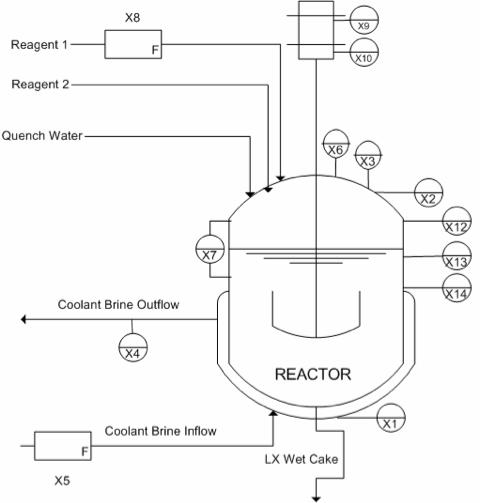
\includegraphics[width=6cm]{images/batch-system.png}	
\end{center}

\end{frame}	

\begin{frame}\frametitle{Batch systems: changing relationship}

	\textbf{Batch system}: group of the \emph{same variables}, gathered over a period of \emph{time}.  Why not just use ordinary PCA or PLS:

	\begin{center}
		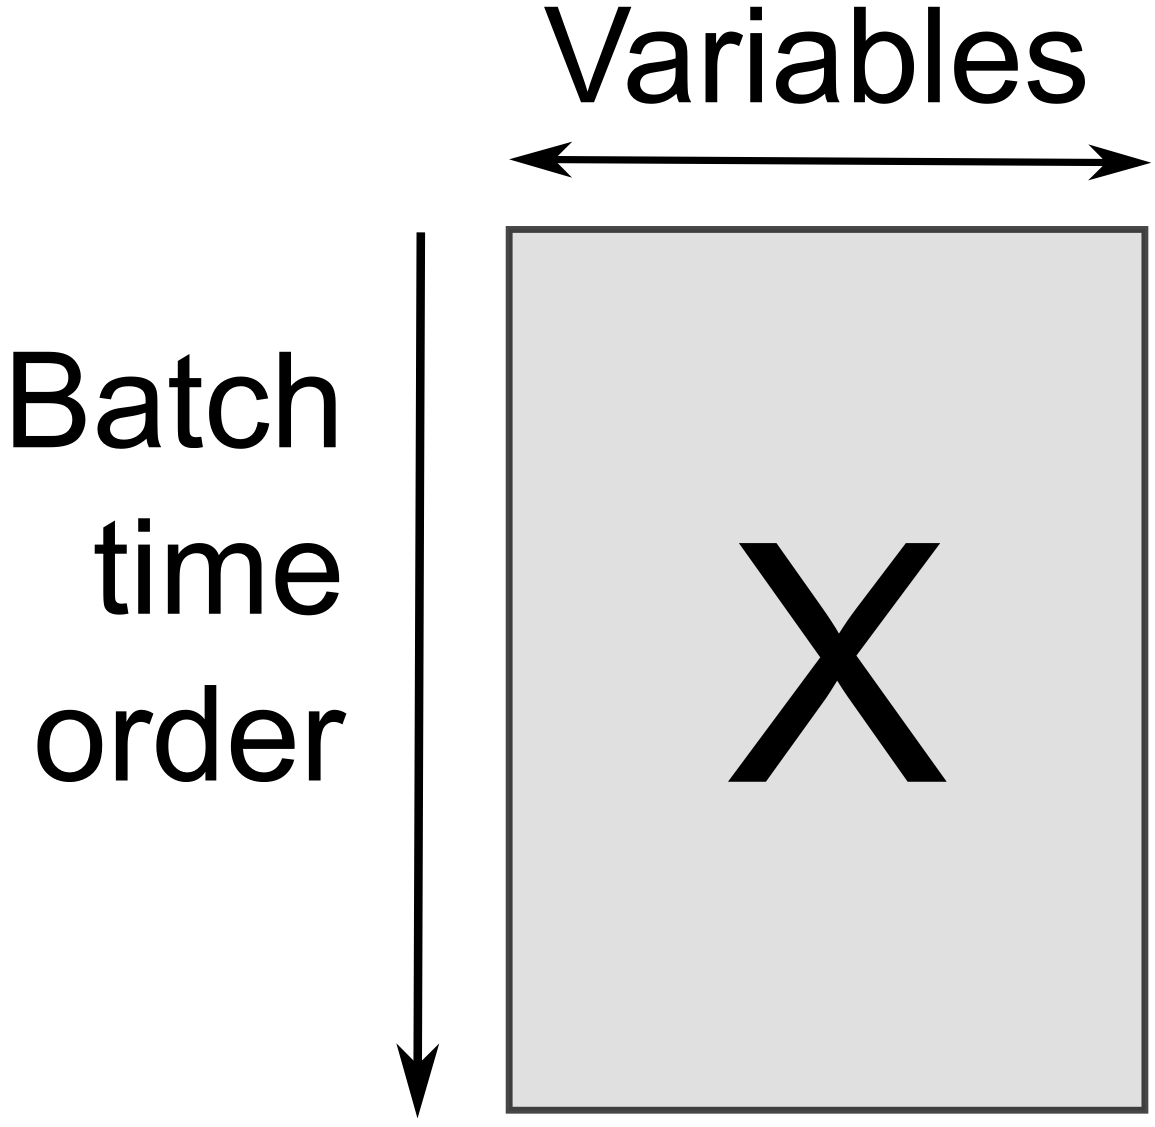
\includegraphics[width=2.4cm]{images/batch-illustrate-unusual-unfolding.png}
	\end{center}


	\begin{itemize}
		\item 	PCA is invariant to row order: 
		\begin{itemize}			
			\item	can shuffle rows, still get same model
			\item 	explain how rows are related to each other
			\item 	each row is assumed independent of the others
			\item 	summarize relationship between variables (columns)
		\end{itemize}
	\end{itemize}

	\begin{exampleblock}{Key issue}
	In \textbf{batch systems}: relationship between variables \alert{changes during the batch}
	\end{exampleblock}
\end{frame}

\begin{frame}\frametitle{Batch systems: changing relationship}

\begin{enumerate}
	\item Relationship between variables change within a batch 
			\begin{itemize}
				\item 	Entry and exit temperatures in a batch dryer correlate (move together) at the end of the batch. 
				\item 	At start of the batch there is little relationship: heat used to evaporate moisture	
			\end{itemize}\pause

	
	\item Past history of a batch affects future behaviour (``integrating system'')
	
			\begin{itemize}
				\item 	Unfold batch data as shown above: cannot capture that ``past effect'' on future rows.  Why?
				\item  	Recall: each row is independent in PCA and PLS
			\end{itemize}

\end{enumerate}
\end{frame}

\begin{frame}\frametitle{Batch systems: changing relationship}
\begin{enumerate}
	\setcounter{enumi}{2}
	\item 	Predictive modelling is harder by unfolding this way

			\begin{center}
				\includegraphics[width=3.5cm]{images/batch-illustrate-unusual-unfolding-with-Y.png}
			\end{center}
			
		
			\begin{itemize}
				\item 	What do we use as the \( \mathbf{Y} \) matrix in this case? {\scriptsize We don't have  \( \mathbf{Y} \) values at each time step.}
				\item 	Many elaborate schemes proposed in literature.			
			\end{itemize}
		
	\item 	Simple solution: arrange data so that each batch is within a row
	
			\begin{itemize}
				\item 	There are some issues with this  (alignment, real-time monitoring)
				\item 	In general, these issues can be addressed effectively
			\end{itemize}
\end{enumerate}
\end{frame}

\begin{frame}\frametitle{Analysis and learning from batch data}

	\begin{exampleblock}{Approach}
	Unfold the aligned batch data row wise, one batch per row, and use PCA and PLS directly.
	\end{exampleblock}

	\begin{center}
		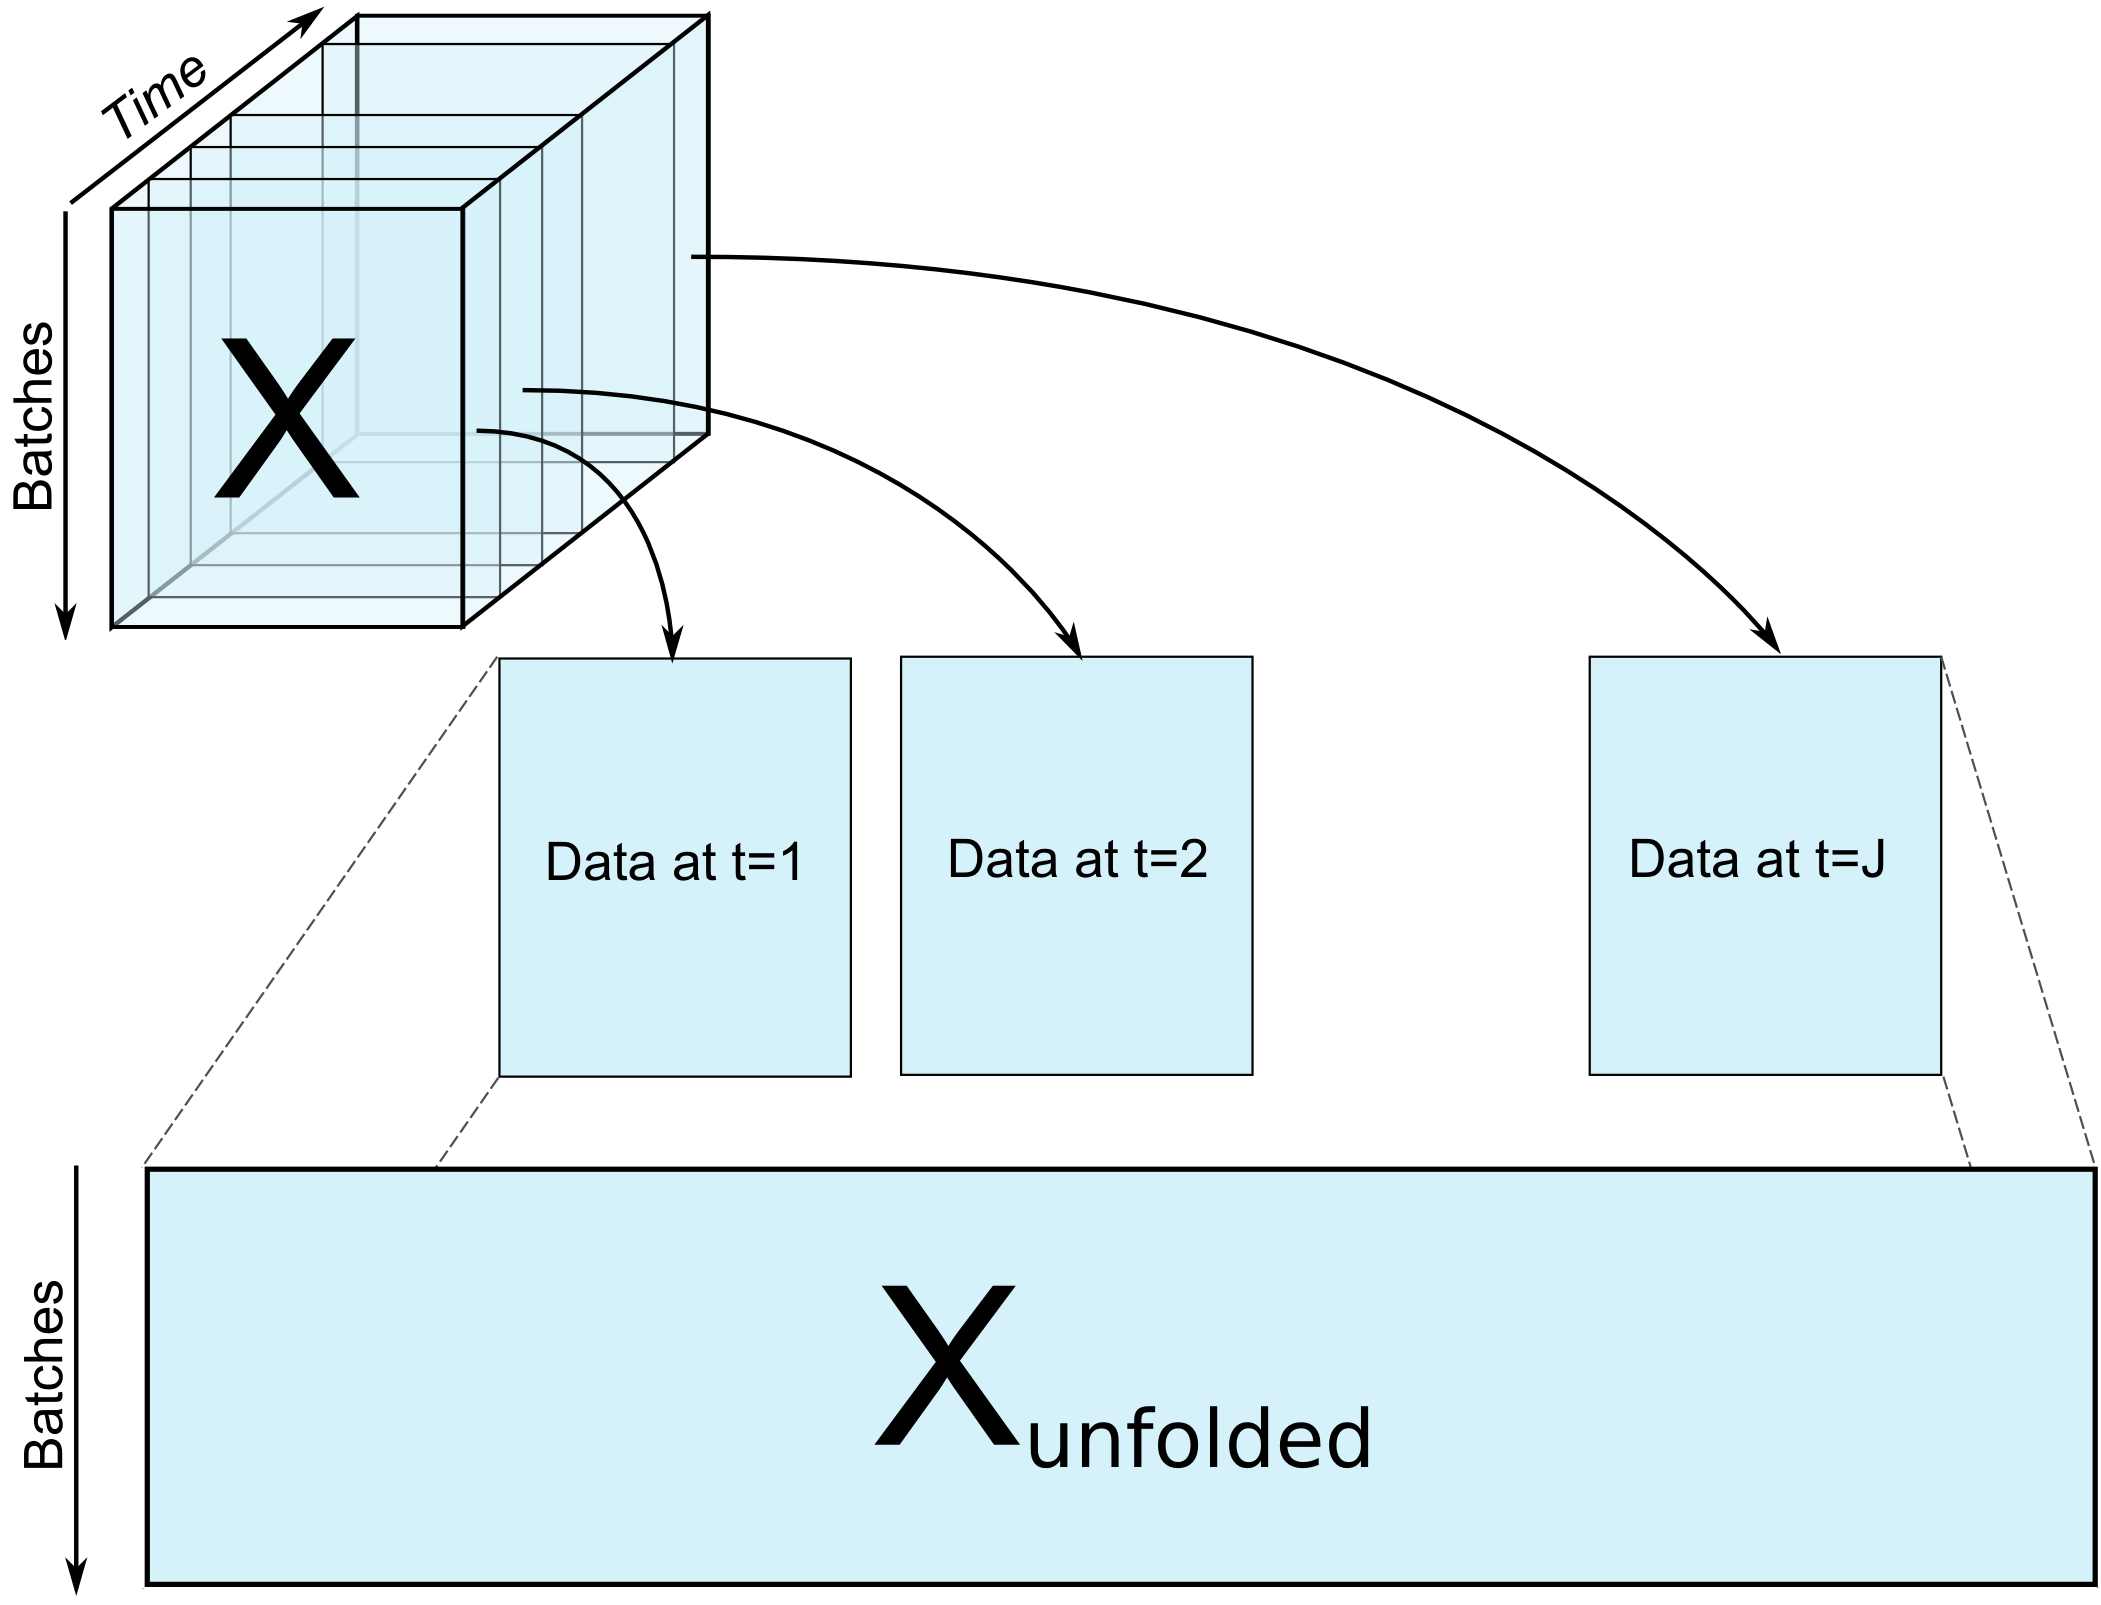
\includegraphics[width=8cm]{images/batch-data-unfolding-X-only.png}	
	\end{center}
\end{frame}	

\begin{frame}\frametitle{DuPont Nylon example: learning from new data}

	\begin{itemize}
		\item	Industrial data set of \( N = 55 \) batches from Nylon production
		
		\item	Temperature, pressure and flow rate variables: \( K = 10\)  batch tags
		
		\item	Batch duration about 2 hours (\( J=100 \) time intervals)
		
		\item	12 hours before lab values returned: batch-to-batch adjustment not possible
		
		\item	Known problems with batches: 40, 41, 42, 50, 51, 53, 54, 55
	\end{itemize}
	
	
\end{frame}

\begin{frame}\frametitle{DuPont Nylon example: raw data}
	{\color{myGreen}{Note}}: data were scaled for confidentiality
	\begin{center}
		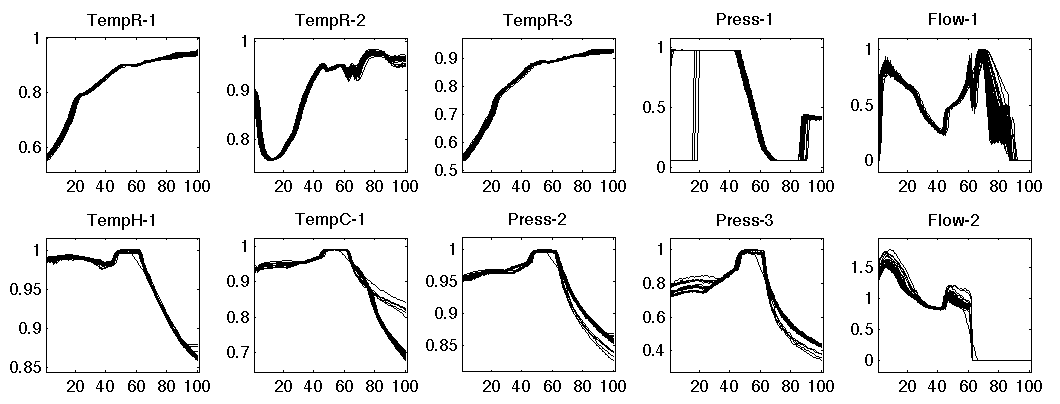
\includegraphics[width=\textwidth]{images/dupont/dupont-raw-data-trajectories.png}
	\end{center}
	
	\vspace{1cm}
	\begin{itemize}
		\item	Can see a few unusual batches: see ``Temp-C1'' and ``Press-1'' tags
		
		\item	Alignment looks pretty good (process is well controlled)
		
		\item	Some periods are noisy: ``Flow-1'' and ``Flow-2''
	\end{itemize}
\end{frame}

\begin{frame}\frametitle{DuPont Nylon example: initial PCA}
	\begin{itemize}

		\item	Just start with 2 components initially
		
				\begin{itemize}					
					\item	no cross-validation, just get a ``feel'' for the data
					\item	\( R^2_X = [38.28\%, 17.58\%]\), or cumulatively: 55.9\%
				\end{itemize}
		
		\item	Score plot:
				
				\begin{columns}
					\column{0.8\textwidth}
						\begin{center}
							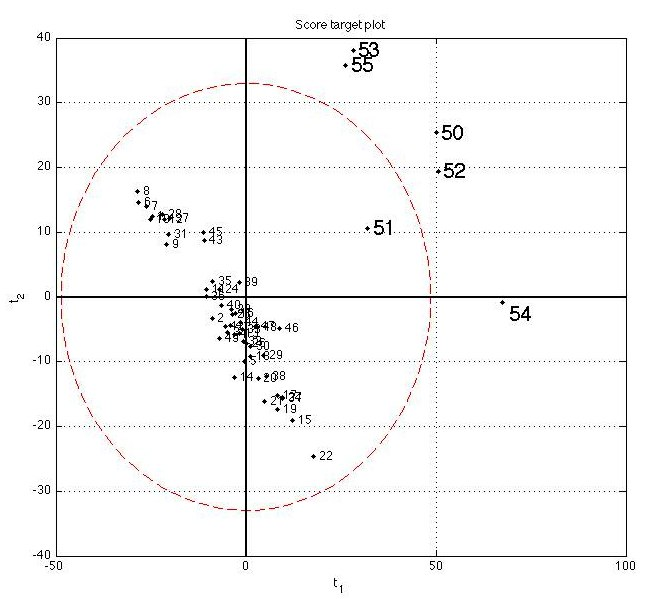
\includegraphics[width=0.8\textwidth]{images/dupont/dupont-raw-score-plot.jpg}
							% batch_PCA = lvm({'X', batch_X}, 2);
							% plot(batch_PCA, 'scores', {'labels'})
						\end{center}
						
					\column{0.4\textwidth}
						\begin{itemize}
							\item	Batches 50 to 55 unusual
							
							\item	Distorted the model		
							
							\item	Before excluding them and rebuilding model, let's first examine them.
						\end{itemize}
				\end{columns}
	\end{itemize}
\end{frame}

\begin{frame}\frametitle{DuPont Nylon example: initial PCA}
	\begin{itemize}
		\item	SPE plot
	\end{itemize}
	
	\begin{center}
		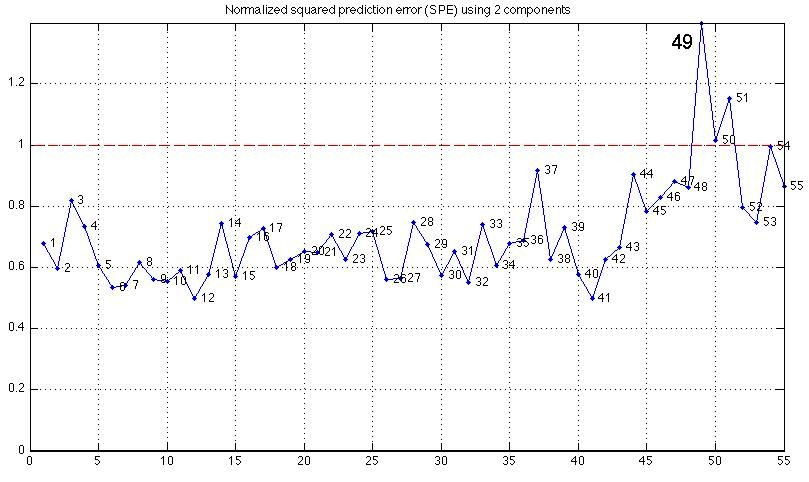
\includegraphics[width=\textwidth]{images/dupont/dupont-raw-SPE.jpg}
		% batch_PCA = lvm({'X', batch_X}, 2);
		% plot(batch_PCA, 'spe', {'labels'})
	\end{center}
\end{frame}

\begin{frame}\frametitle{DuPont Nylon example: batch 54 (high \( t_1 \) batch)}
	\begin{itemize}
		\item	Contribution plot in \( t_1 \)
	\end{itemize}
	
	\begin{center}
	\end{center}
\end{frame}

\begin{frame}\frametitle{DuPont Nylon example: Summary}
	
\begin{enumerate}
	\item	Plot the trajectories
	
			\begin{itemize}
				\item	Sometime outlier batches already detectable
				
				\item	Visualize how good your alignment is: do data need extra pretreatment?
			\end{itemize}
\end{enumerate}


	
\end{frame}

